\section{SCL object model}

\todo[inline]{en algun lado debo hablar de los conceptos
de SCL, que es, explicar de que es un lenguaje basado en xml, y 
que su estructura esta descripta en los XSDs definidos 
en la parte 6 de la norma}

As explained in section \ref{fig:pdf-SCL-uml-deept2} \todo{completar bien la referencia}, 
the SCL describes the SAS by modelling objects.
The standard IEC 61850-6 \cite{IEC61850-6:2004} object model 
structure and constraints are described in terms of the 
Schema Definition Language (XSD) \todo{abreviacion, corregir}.

The XSD of the SCL are structured as depicted 
in the figure \href{fig:pdf-SCL-uml-deept2}. 
Basically, it is composed by: 
\todo[color=green!40]{61850, parte6, cl6.1, \textparagraph 5}

\begin{itemize}
  \item The substation model: the object model of the primary power structure
  		(a instance of tSubstation) with their designations structured according to 
  		IEC 61346-1 \cite{IEC61346-1:1996}. 
  \item The communication model: the object model of the IED 
  		communication system configuration, 
  		i.e.,
  		the the networks, subnetworks, ports informations
  		\todo[color=green!40]{61850, parte6, cl6.1, \textparagraph 5},
  		the communication connection relations of IEDs to 
  		subnetworks, the routing for another subnetworks informations, 
  		and clocks configuration information and locations for 
  		time synchronisation (the gateways are not considered here, 
  		a gateway has to be modelled as another IED)
  		\todo[color=green!40]{61850, parte6, cl6.1, \textparagraph 8}.
  \item The product model: Contains the IEDs objects and their 
  		logical node implementations. 	
\end{itemize}

\section{SCL modelling steps}
\todo[inline]{esta seccion la dejo pendiente,
debo escribirlo con detenimiento para 
que queden en concordancia la 
figura \ref{fig:pdf-SCL-uml-deept2} 
y lo que tengo escrito en esta seccion}
The more usual approach for the \gls{SAS} description 
with \gls{SCL} begin with the 
single line drawing process where the 
substation topology are defined using a 
system configurator tool. The system configurator tool, 
described in the section \ref{sec:ch-scl--System-configurator-tool}, 
creates the \gls{SSD} file containing the \gls{LNodes}
and their allocation in the substation.

The \glspl{LNode} object SCL models (from the substation section) 
is used to map 
The \gls{IED} object model that describes 
the \gls{IED} objects are used to mapping  

\todo[inline]{debo agregar aca la explicacion de los demas modelos
descriptos mediance los XSDs, pues esos tres 
items que menciona la norma son solo los mas
importantes, pero no da para entender y saber leer 
los archivos scl sabiendo solo eso. Los tres items mencionados arriba
son solo la base. Falta principalmente el DATypeTemplate
que corresponden a los objetos a serializar correspondientes 
a las instancias de las clases de la parte 7-x}

\begin{landscape}
	\begin{figure}
	  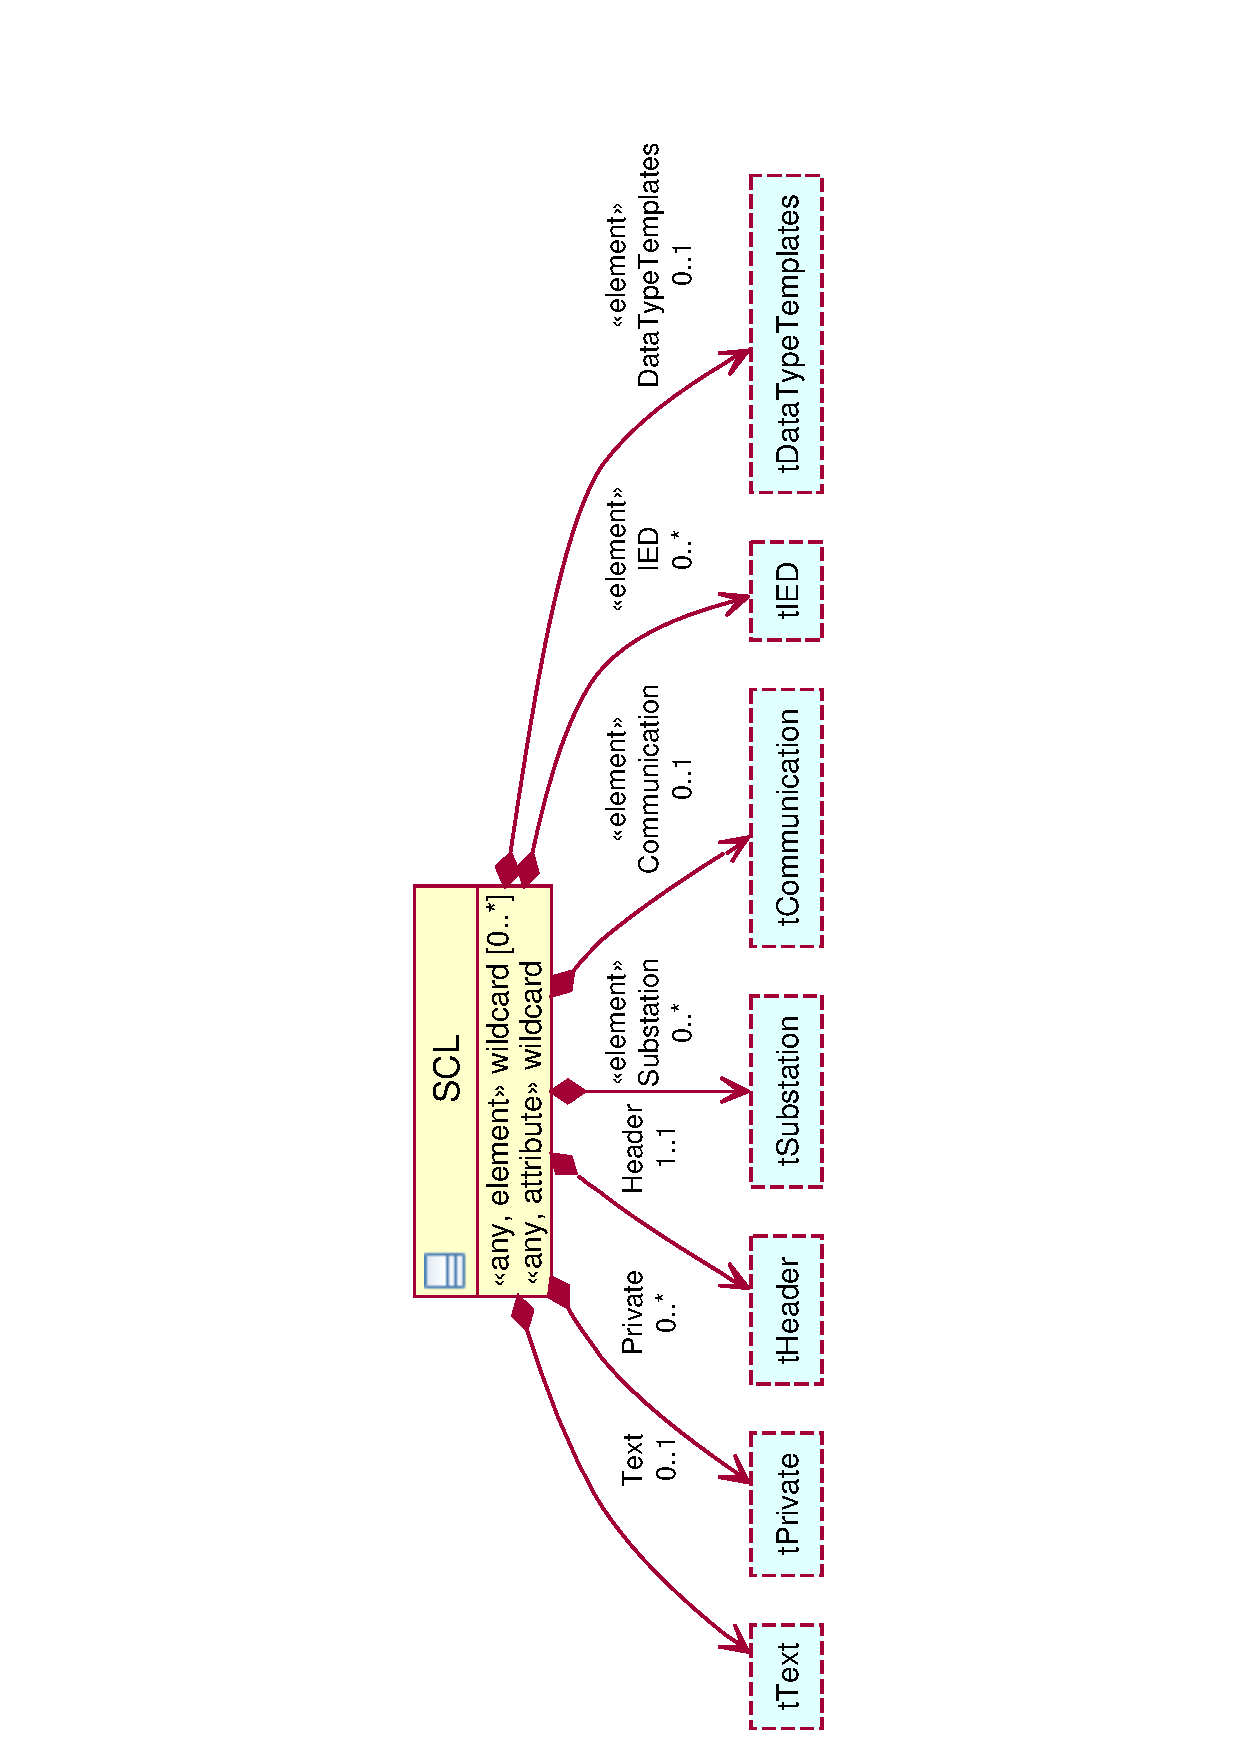
\includegraphics[angle=-90, width=1.0\linewidth]{chapters/ch-scl/figures/SCL-uml-Deept2}
	  \caption{SCL object model}  
	  \label{fig:pdf-SCL-uml-deept2}
	\end{figure}
\end{landscape}


\begin{landscape}
	\begin{figure}
	  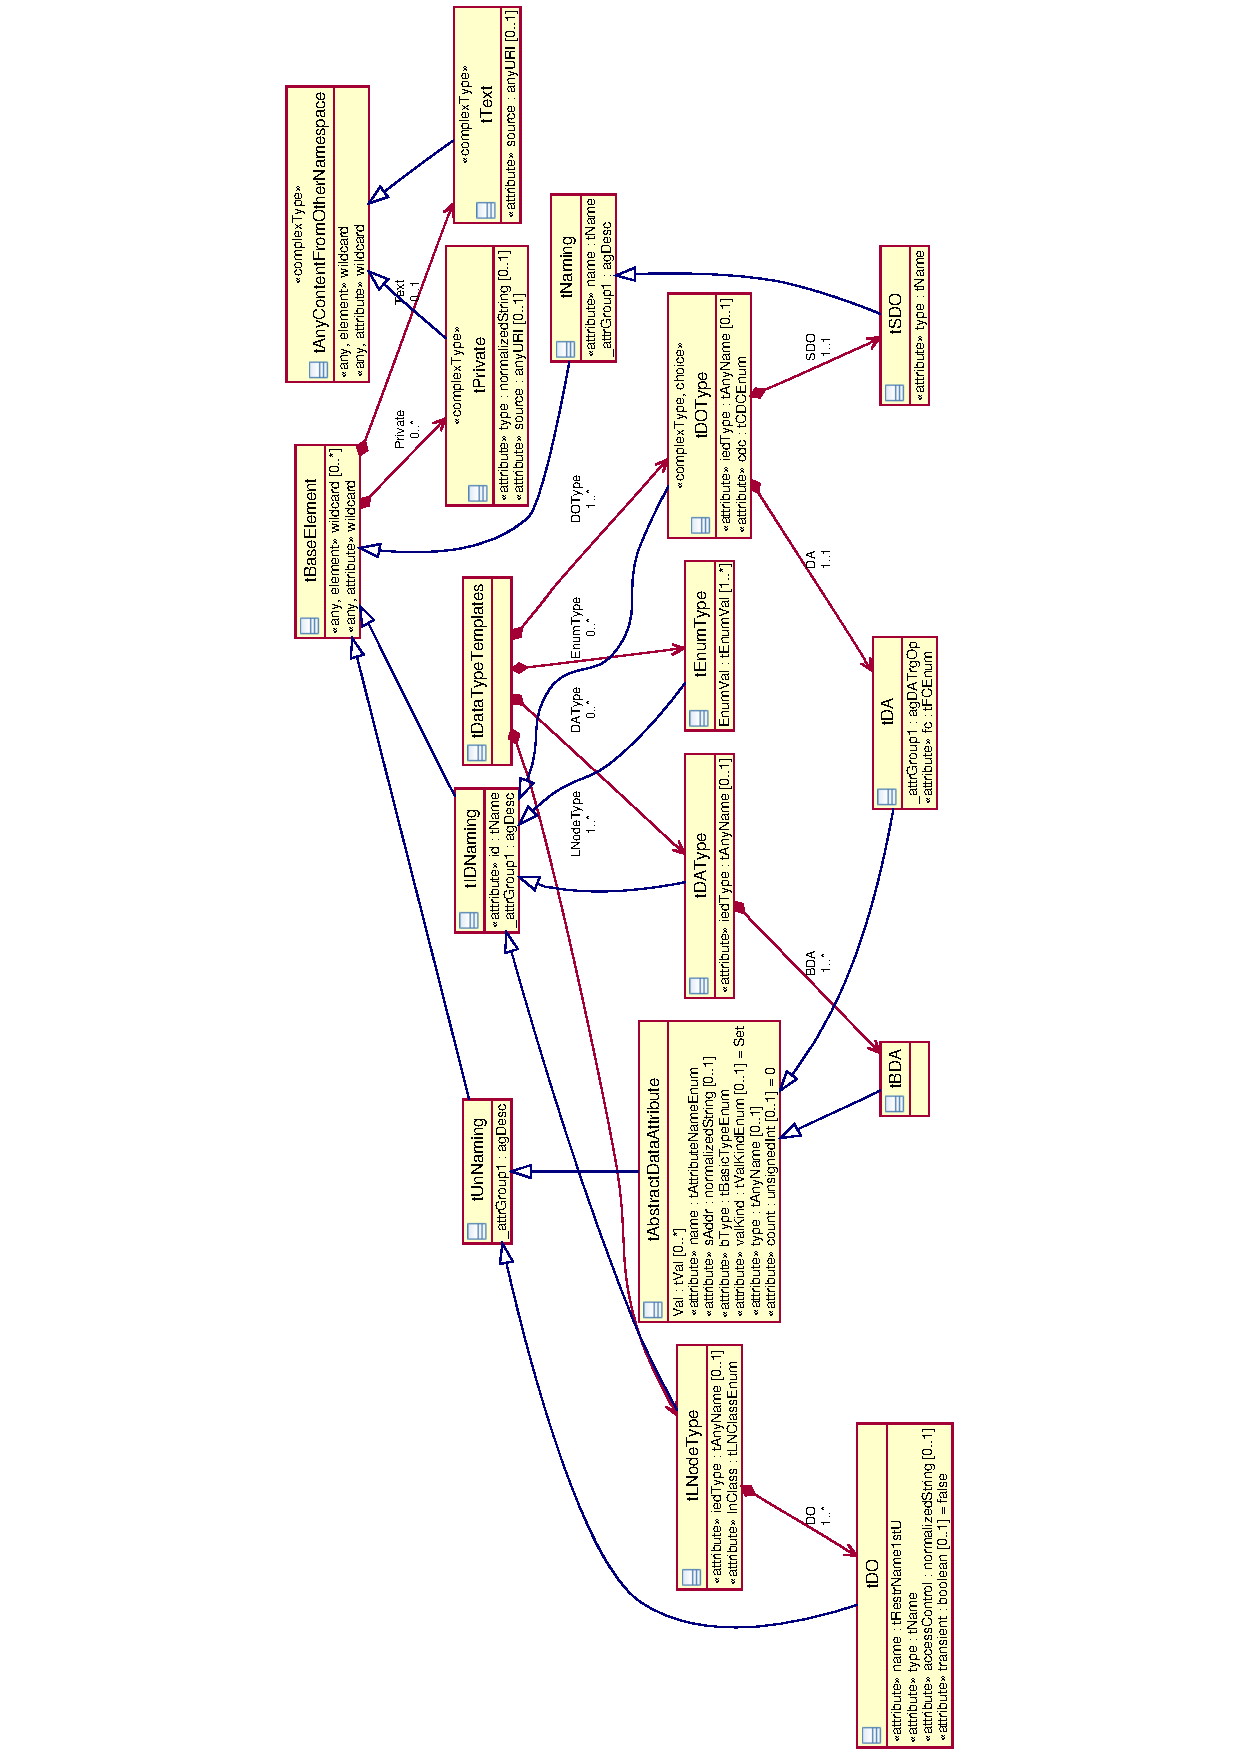
\includegraphics[angle=-90, width=1.0\linewidth]{chapters/ch-scl/figures/SCL-uml-DATypeTemplate-Deept2}
	  \caption{DAType object model template with heritance details}  
	  \label{fig:pdf-SCL-uml-DATypeTemplate-Deept2}
	\end{figure}
\end{landscape}

\begin{landscape}
	\begin{figure}
	  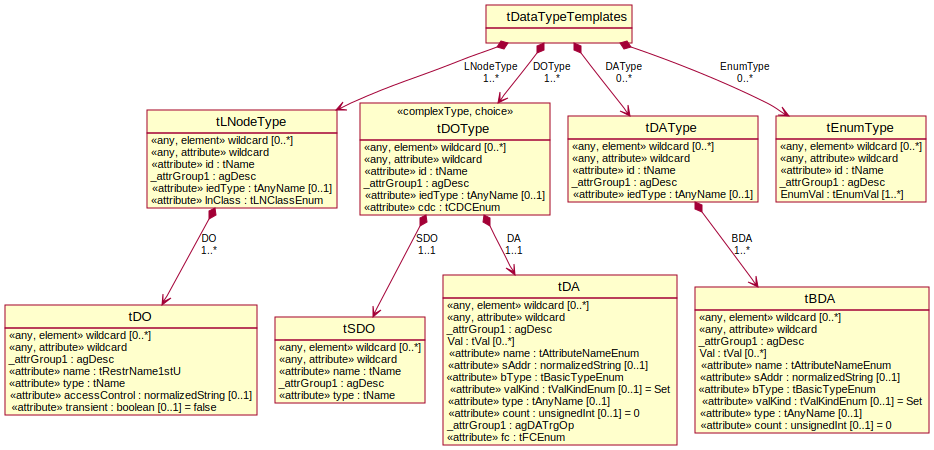
\includegraphics[angle=-90, width=1.0\linewidth]{chapters/ch-scl/figures/SCL-uml-DATypeTemplate-Deept2-inherited}
	  \caption{DAType object model template inherited}  
	  \label{fig:pdf-SCL-uml-DATypeTemplate-Deept2-inherited}
	\end{figure}
\end{landscape}

\begin{landscape}
	\begin{figure}
	  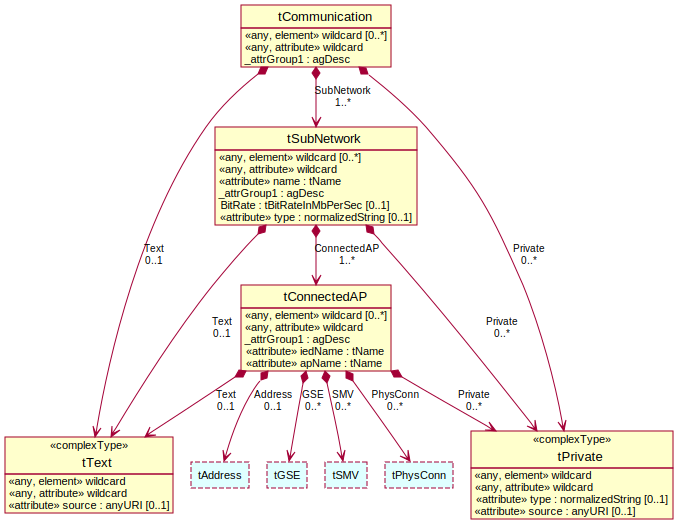
\includegraphics[angle=-90, width=1.0\linewidth]{chapters/ch-scl/figures/SCL-uml-communication-Deept3}
	  \caption{SCL Communication object model}  
	  \label{fig:pdf-SCL-uml-communication-Deept3}
	\end{figure}
\end{landscape}

\todo[inline]{podria convenir cambiar la palabra object model por class diagram
en todos estos graficos}

\todo[inline]{a este le valta
expandir la clase correspondiente hasta que muestre el transformador }
\begin{figure}
  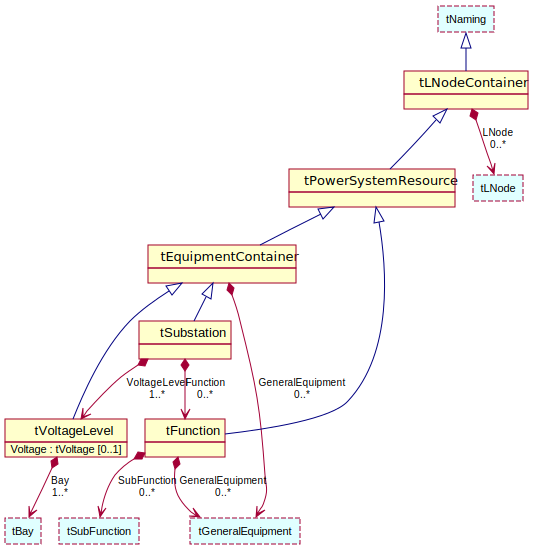
\includegraphics[width=1.0\linewidth]{chapters/ch-scl/figures/SCL-uml-substation-Deept2}
  \caption{SCL Substation object model with heritance 
  details  } 
  \label{fig:pdf-SCL-uml-substation-Deept2}
\end{figure}


\todo[inline]{a este le valta
  expandir la clase correspondiente hasta que muestre el transformador }
\begin{figure}
  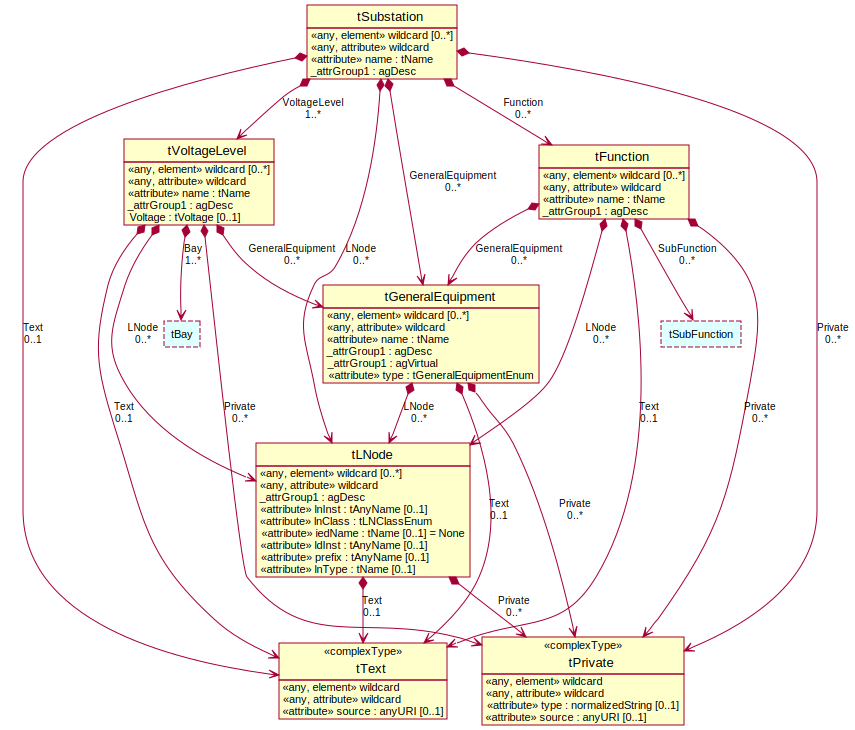
\includegraphics[width=1.0\linewidth]{chapters/ch-scl/figures/SCL-uml-substation-Deept2-inherited}
  \caption{SCL Substation object model inherited  }
  \label{fig:pdf-SCL-uml-substation-Deept2-inherited}
\end{figure}

The UML of the 
figure \ref{fig:SCL-uml-Resumen} 
is a resume of
the SCL model, where is evident the 
key importance of the Logical Node for  
the information topology description (see 
the composition of the Substation 
class). The Logical Node is  
the transition object to 
connect the diferent structures of the SAS 
\todo[color=green!40]{61850, parte6, cl6.1, \textparagraph 9} 
that are defined by IEC 61341-1 \cite{IEC61346-1:1996}.


\begin{landscape}

\begin{figure}
  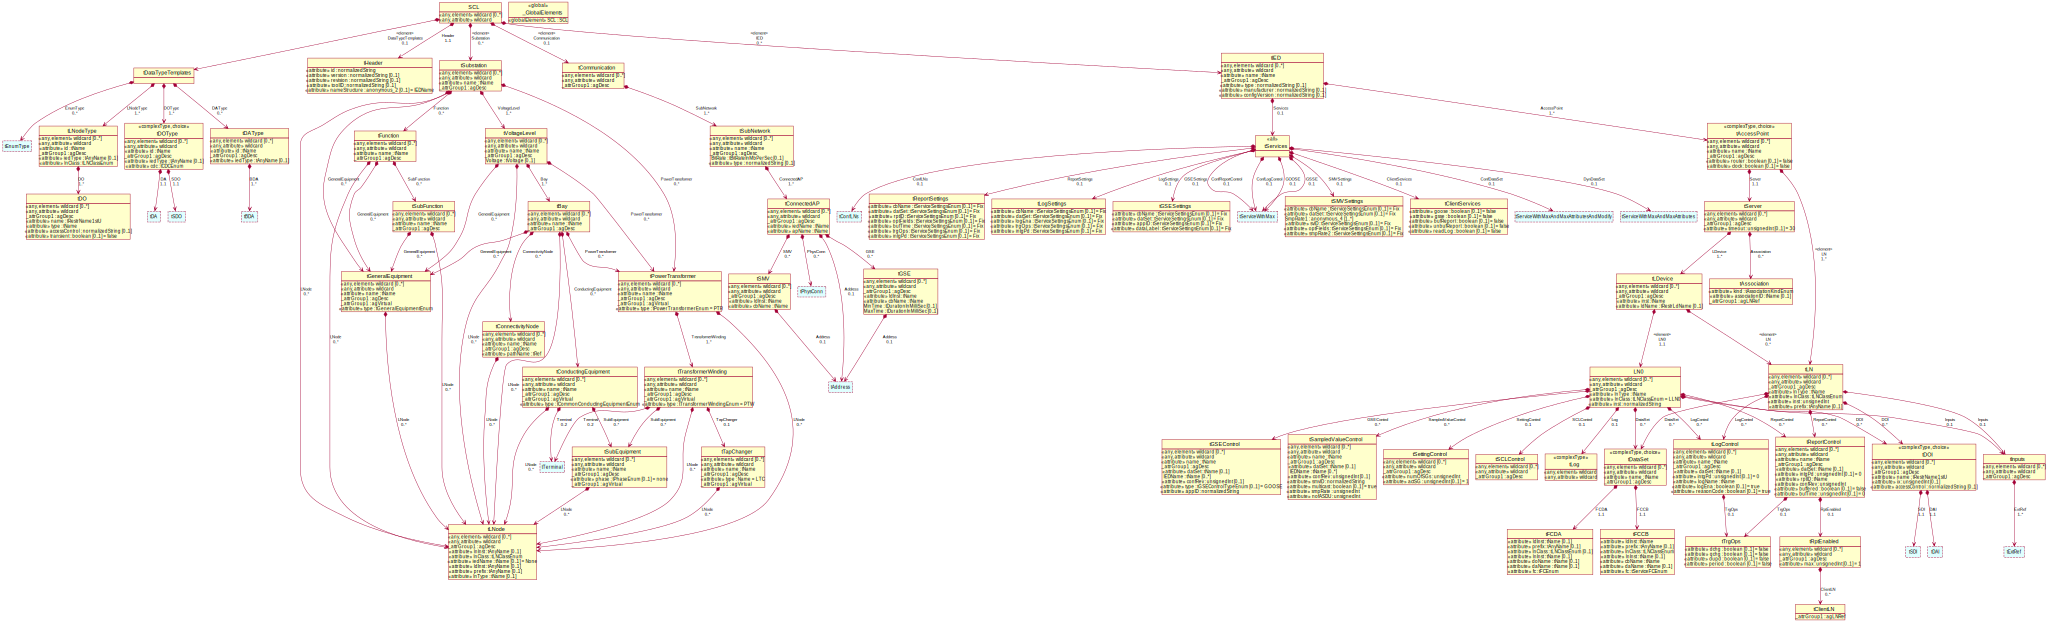
\includegraphics[angle=-90,
  width=1.0\linewidth]{chapters/ch-scl/figures/SCL-uml-Resumen-inherited}
  \caption{Resume of SCL shema represented by a UML class diagram}
  \label{fig:SCL-uml-Resumen}
\end{figure}
\end{landscape}
